\documentclass{standalone}
% Preamble
\begin{document}

  \section{Expérimentation}
  Nous choisissons $n=
\input{../txt/n.txt}
$ et le multidegré $
\input{../txt/deg.txt}
$. La matrice de Bezout $B(1)$, à coefficients entiers, est de taille \input{../txt/Dx.txt},
   \begin{center}
  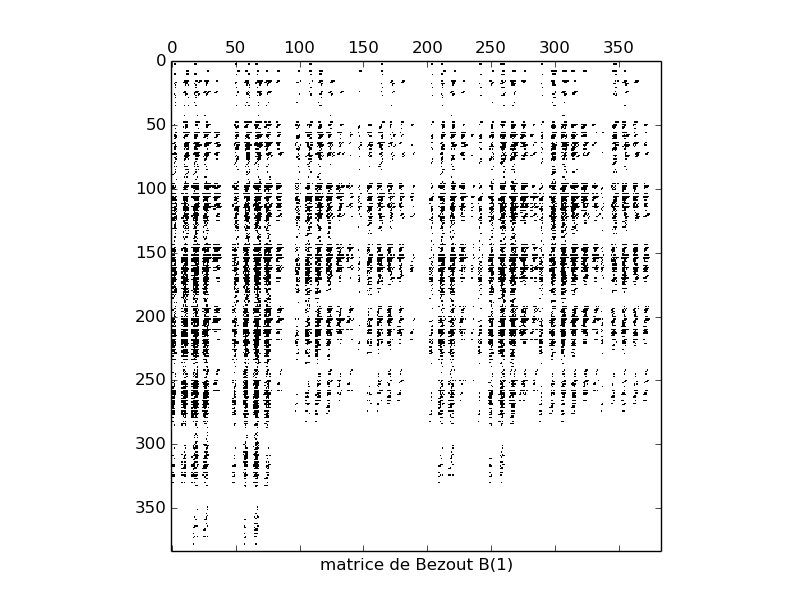
\includegraphics[width=8cm]{../png/bez.png}
  \end{center}


  En permutant lignes et colonnes on obtient une matrice bloc-triangulaire supérieure
   \begin{center}
  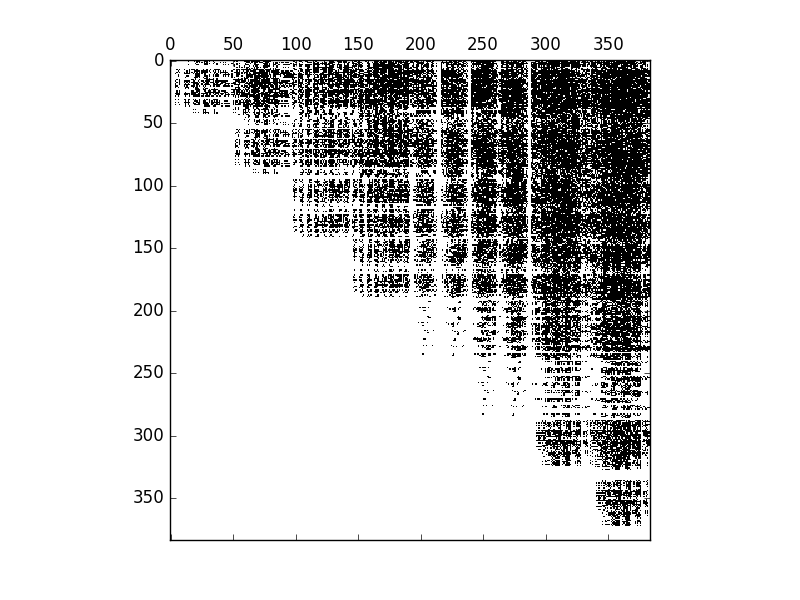
\includegraphics[width=8cm]{../png/beztri.png}
  \end{center}
  dont on peut calculer le noyau plus facilement. On trouve que rang de $B(1)$ vaut \input{../txt/dim0.txt}.
  Une fois le processus de réduction terminé on obtient des matrices $B(1), B(x_j), j=1,\cdots,n$ de même taille, $B(1)$ étant inversible. On trouve que la dimension de $A$ est \input{../txt/dim.txt}. Les matrices compagnon $X_j = B(x_j)B(1)^{-1}$ fournissent alors les racines du système polynômial. Pour chacune des racines obtenues nous vérifions sa qualité en lui appliquant les polynômes $f_i, i=1,\cdots,n$ puis on représente en graphique semi-logarithmique la  valeur absolue du résultat. Les mêmes résultats représentés sous forme d'histogramme
   \begin{center}
  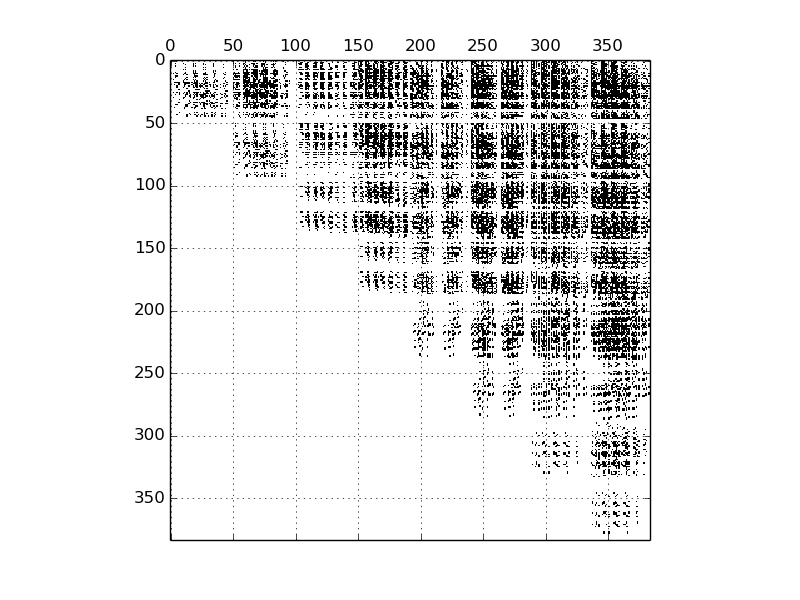
\includegraphics[height=10cm, width=18cm]{../png/ref.png}
  \end{center}

  Dans cet exemple nous voyons que la qualité est excellente pour toutes les racines.

\end{document}
